%%%%%%%%%%%%%%%%%%%%%%%%%%%%%%%%%%%%%%%%%%%%%%%%%%%%%%%%%%%%%%%%%%%%%%%%%%%%%%%%%%%%%%%%%%%%%%%%%%%%%%%%%%%%%%%%%%%%%%%%%%%%%%%%%%%%%%%%%%%%%%%%%%%%%%%%%%%%%%%%%%%
% Written By Michael Brodskiy
% Class: Fundamentals of Linear Systems
% Professor: I. Salama
%%%%%%%%%%%%%%%%%%%%%%%%%%%%%%%%%%%%%%%%%%%%%%%%%%%%%%%%%%%%%%%%%%%%%%%%%%%%%%%%%%%%%%%%%%%%%%%%%%%%%%%%%%%%%%%%%%%%%%%%%%%%%%%%%%%%%%%%%%%%%%%%%%%%%%%%%%%%%%%%%%%

\include{Includes.tex}

\title{Homework 3}
\date{\today}
\author{Michael Brodskiy\\ \small Professor: I. Salama}

\begin{document}

\maketitle

\begin{enumerate}

  \item Classifying systems as memory-less, time-invariant, linear, causal, and/or stable:

    \begin{enumerate}

      \item $y(t)=5e^{4t}x(t-1)$

        \begin{itemize}

          \item Memory: \textbf{not} memory-less; the $x(t-1)$ term means the system relies on values other than the present value; therefore, it is not memory-less

          \item Time-Invariant: \textbf{not} time-invariant; we may see that, $y(t-t_o)$ changes the $t$ value in the exponential and $x(t)$ statement, while $x(t-t_o)$ changes only the $x(t)$ statement; thus, it is not time-invariant, since $x(t-t_o)\neq y(t-t_o)$

          \item Linear: the system \textbf{is} linear (see below) because $ax_1(t)+bx_2(t)= ay_1(t)+by_2(t)$

            $$ax_1(t)+bx_2(t)\to a5e^{4t}x_1(t-1)+b5e^{4t}x_2(t-1)$$
            $$ay_1(t)+by_2(t)\to a5e^{4t}x_1(t-1)+b5e^{4t}x_2(t-1)$$

          \item Causal: the system \textbf{is} causal , because it only depends on past or present values (ex. $t=0\to y(t)=5e^{4(0)}x(-1)$)

          \item Stable: Given that the system depends on an exponential $e^{4t}$, its maximum value is unbounded and, therefore, it is \textbf{unstable}

        \end{itemize}

      \item $y(t)=\displaystyle \int_{-\infty}^{\frac{t}{2}} x(\tau)\,d\tau$

        \begin{itemize}

          \item Memory: \textbf{not} memory-less; the system depends on a shift of the $t$ parameter ($t/2$), and, therefore, does not always depend on the current value of time

          \item Time-Invariant: \textbf{not} time-invariant; $y(t-t_o)\neq x(t-t_o)$ (see below)

            $$x(t-t_o)\to \int_{-\infty}^{\frac{t}{2}} x(\tau-t_o)\,d\tau$$
            $$y(t-t_o)\to \int_{-\infty}^{\frac{(t-t_o)}{2}} x(\tau-t_o)\,d\tau$$
            $$\therefore x(t-t_o)\neq y(t-t_o)$$

          \item Linear: the system \textbf{is} linear; it follows both the superposition and homogeneity principles (see below)

            $$ay_1(t)+by_2(t)\to a\int_{-\infty}^{\frac{t}{2}} x_1(\tau)\,d\tau+b\int_{-\infty}^{\frac{t}{2}} x_2(\tau)\,d\tau$$
            $$ax_1(t)+bx_2(t)\to a\int_{-\infty}^{\frac{t}{2}} x_1(\tau)\,d\tau+b\int_{-\infty}^{\frac{t}{2}} x_2(\tau)\,d\tau$$
            $$\therefore ax_1(t)+bx_2(t)=ay_1(t)+by_2(t)$$

          \item Causal: the system \textbf{is not} causal; integration depends on future values when $t<0$

          \item Stable: the system \textbf{is not} stable (see below)

            $$y(t)=\int_{-\infty}^{\frac{t}{2}} x(\tau)\,d\tau$$
            $$h(t)=\int_{-\infty}^{\frac{t}{2}} \delta(\tau)\,d\tau=\left\{\begin{array}{ll}0,& t<0\\1,& t>0\end{array}$$
            $$h(t)\to u(t)$$
            $$\int_{-\infty}^{\infty} h(t)\,dt=\infty$$

        \end{itemize}

      \item $y(t)=4+5\dfrac{d^2}{dt^2}x(t)$

        \begin{itemize}

          \item Memory: the system is \textbf{not} memory-less; the use of a differential implies that the system depends on past values

          \item Time-Invariant: the system \textbf{is} time-invariant (see below)

            $$x(t-t_o)\to 4+5\dfrac{d^2}{dt^2}x(t-t_o)$$
            $$y(t-t_o)\to 4+5\dfrac{d^2}{dt^2}x(t-t_o)$$
            $$\therefore x(t-t_o)=y(t-t_o)$$

          \item Linear: the system is \textbf{not} linear (see below)

            $$ax_1(t)+bx_2(t)=\left(4+5a\dfrac{d^2}{dt^2}x_1(t)\right)+\left(4+5b\dfrac{d^2}{dt^2}x_2(t)\right)$$
            $$ay_1(t)+by_2(t)=a\left(4+5\dfrac{d^2}{dt^2}x_1(t)\right)+b\left(4+5\dfrac{d^2}{dt^2}x_2(t)\right)$$
            $$\therefore ax_1(t)+bx_2(t)\neq ay_1(t)+by_2(t)$$

          \item Causal: the system \textbf{is} causal because it only depends on past or present values

          \item Stable: the system is \textbf{unstable} because it is unbounded

        \end{itemize}

      \item $y(t)=\left\{\begin{array}{ll} 0, & t<0\\ x(t-2)+2x(t), & t\geq0\end{array}$

        \begin{itemize}

          \item Memory: the system is \textbf{not} memory-less, since the $x(t-2)$ term depends on a past value

          \item Time-Invariant: the system is \textbf{not} time-invariant (see below)

            $$x(t-t_o)\to\left\{\begin{array}{ll} 0, & t<0\\ x(t-2-t_o)+2x(t-t_o), & t\geq0\end{array}$$
            $$y(t-t_o)\to\left\{\begin{array}{ll} 0, & t<2\\ x(t-2-t_o)+2x(t-t_o), & t\geq2\end{array}$$
            $$\therefore x(t-t_o)\neq y(t-t_o)$$

          \item Linear: the system \textbf{is} linear (see below)

            $$ax_1(t)+bx_2(t)\to\left\{\begin{array}{ll} 0, & t<0\\ ax_1(t-2)+2ax_1(t)+bx_2(t-2)+2bx_2(t), & t\geq0\end{array}$$
            $$ay_1(t)+by_2(t)\to\left\{\begin{array}{ll} 0, & t<0\\ ax_1(t-2)+2ax_1(t)+bx_2(t-2)+2bx_2(t), & t\geq0\end{array}$$
              $$\therefore ax_1(t)+bx_2(t)=ay_1(t)+by_2(t)$$

            \item Causal: the system \textbf{is} causal because it only depends on past or present values

            \item Stable: the system \textbf{is} stable, because it does not tend to diverge

        \end{itemize}

        Problem 1 can be tabulated as follows:

        \begin{center}
          \begin{tabular}[H]{|c|c|c|c|c|}
            \hline
            System & a & b & c & d\\
            \hline
            Memory-Less & no & no & no & no\\
            \hline
            Time-Invariant & no & no & yes & no\\
            \hline
            Linear & yes & yes & no & yes\\
            \hline
            Causal & yes & no & yes & yes\\
            \hline
            Stable & no & no & no & yes\\
            \hline
          \end{tabular}
        \end{center}

    \end{enumerate}

  \item Classifying systems as memory-less, time-invariant, linear, causal, and/or stable:

    \begin{enumerate}

      \item $y[n]=x[n+1]-2x[n-4]$

        \begin{itemize}

          \item Memory: system is \textbf{not} memory-less, as it depends on past and future values

          \item Time-Invariant: system \textbf{is} time-invariant (see below)

            $$x[n-n_o]=x[n+1-n_o]-2x[n-4-n_o]$$
            $$y[n-n_o]=x[n+1-n_o]-2x[n-4-n_o]$$
            $$\therefore x[n-n_o]=y[n-n_o]$$

          \item Linear: system \textbf{is} linear (see below)

            $$ax_1[n]+bx_2[n]=a(x_1[n+1]-2x_1[n-4])+b(x_2[n+1]-2x_2[n-4])$$
            $$ay_1[n]+by_2[n]=a(x_1[n+1]-2x_1[n-4])+b(x_2[n+1]-2x_2[n-4])$$
            $$\therefore ay_1[n]+by_2[n]=ax_1[n]+bx_2[n]$$

          \item Causal: system is \textbf{not} causal, as it depends on past and present values

          \item Stable: system \textbf{is} stable because $y[n]$ is finite

        \end{itemize}

      \item $y[n]=\text{Even}\left\{ x[n-1] \right\}$

        To simplify analysis, we can express the even function as:

        $$\frac{x[n]+x^*[-n]}{2}\to\frac{x[n-1]+x^*[-n+1]}{2}$$

        \begin{itemize}

          \item Memory: system is \textbf{not} memory-less, as it depends on future values

          \item Time-Invariant: system \textbf{is} time-invariant (see below)

            $$x[n-n_o]=\text{Even}\left\{ x[n-1-n_o] \right\}$$
            $$y[n-n_o]=\text{Even}\left\{ x[n-1-n_o] \right\}$$
            $$\therefore x[n-n_o]=y[n-n_o]$$

          \item Linear: system is \textbf{not} linear (see below); note that this is because $a$ or $b$ may be complex. Given this, for a purely real signal, the system can be classified as linear; however, due to the need to use the 'conjugate' for the even function, in the case of a complex signal, this is non-linear

            $$ax_1[n]+bx_2[n]=\frac{ax_1[n-1]+a^*x_1^*[-n+1]}{2}+\frac{bx_2[n-1]+b^*x_2^*[-n+1]}{2}$$
            $$ay_1[n]+by_2[n]=\frac{ax_1[n-1]+ax_1^*[-n+1]}{2}+\frac{bx_2[n-1]+bx_2^*[-n+1]}{2}$$
            $$\therefore ay_1[n]+by_2[n]\neq ax_1[n]+bx_2[n]$$

          \item Causal: system is \textbf{not} causal, as it depends on a future value

          \item Stable: system \textbf{is} stable because $y[n]$ is finite

        \end{itemize}

      \item $y[n]=5x[3n+1]$

        \begin{itemize}

          \item Memory: system is \textbf{not} memory-less, as it depends on non-present values

          \item Time-Invariant: system is \textbf{not} time-invariant (see below)

            $$x[n-n_o]=5x[3n-n_o+1]$$
            $$y[n-n_o]=5x[3n-3n_o+1]$$
            $$\therefore x[n-n_o]\neq y[n-n_o]$$

          \item Linear: system \textbf{is} linear (see below)

            $$ax_1[n]+bx_2[n]=5ax_1[3n+1]+5bx_2[3n+1]$$
            $$ay_1[n]+by_2[n]=5ax_1[3n+1]+5bx_2[3n+1]$$
            $$\therefore ay_1[n]+by_2[n]=ax_1[n]+bx_2[n]$$

          \item Causal: system is \textbf{not} causal, as it depends on a future value

          \item Stable: system \textbf{is} stable because $y[n]$ is finite

        \end{itemize}

      \item $y[n]=\left\{ \begin{array}{ll} 0, & n=2\\ x[n], & \text{otherwise}\end{array}$

        \begin{itemize}

          \item Memory: system \textbf{is} memory-less; it does not depend on past or present values

          \item Time-Invariant: system is \textbf{not} time-invariant (see below)

            $$x[n-n_o]=\left\{ \begin{array}{ll} 0, & n=2\\ x[n-n_o], & \text{otherwise}\end{array}$$
            $$y[n-n_o]=\left\{ \begin{array}{ll} 0, & n=2+n_o\\ x[n-n_o], & \text{otherwise}\end{array}$$
            $$\therefore x[n-n_o]\neq y[n-n_o]$$

          \item Linear: system \textbf{is} linear (see below)

            $$ax_1[n]+bx_2[n]=\left\{ \begin{array}{ll} 0, & n=2\\ ax_1[n]+bx_2[n], & \text{otherwise}\end{array}$$
            $$ay_1[n]+by_2[n]=\left\{ \begin{array}{ll} 0, & n=2\\ ax_1[n]+bx_2[n], & \text{otherwise}\end{array}$$
            $$\therefore ay_1[n]+by_2[n]=ax_1[n]+bx_2[n]$$

          \item Causal: system \textbf{is} causal, as it depends on only past or present values

          \item Stable: system \textbf{is} stable because $y[n]$ is finite

        \end{itemize}

    \end{enumerate}

  \item

    \begin{enumerate}

      \item 

        We may begin by constructing the expression for the convolution sum:

        $$y[n]=\sum_{k=-\infty}^{\infty}x[k]h[n-k]$$

        This gets us:

        $$y[n]=\sum_{k=-\infty}^{\infty} \left( \frac{1}{4} \right)^{k-2}u[k-2]u[n-k+1]$$

        We may observe the following:

        $$x[n]\neq 0,\quad n\geq 2$$
        $$h[n]\neq 0,\quad n\geq -1$$

        Integrating this into the convolution sum, we may see that the expression is nonzero (unit functions both exist) for $k\geq 2$, and that $k\leq n+1$. Thus, we get:

        $$y[n]=\sum_{k=2}^{n+1} \left( \frac{1}{4} \right)^{k-2}$$

        Using the expansion for series, we obtain:

        $$y[n]=\frac{1-(.25)^{n-1}}{1-.25}$$
        $$\boxed{y[n]=\frac{4}{3}\left[ 1-\left( \frac{1}{4} \right)^{n-1} \right]\text{ for }n\geq 2}$$\\

        This can be sketched as:

        \begin{figure}[H]
          \centering
          \tikzset{every picture/.style={line width=0.75pt}} %set default line width to 0.75pt        

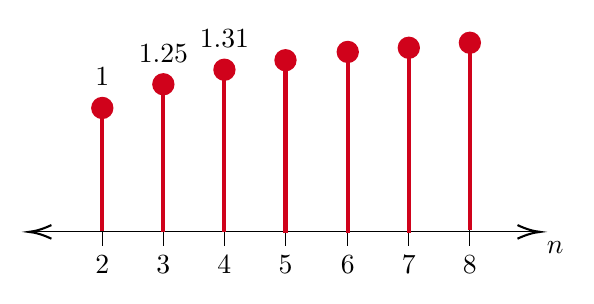
\begin{tikzpicture}[x=0.75pt,y=0.75pt,yscale=-1,xscale=1]
%uncomment if require: \path (0,412); %set diagram left start at 0, and has height of 412

%Straight Lines [id:da8584009914648288] 
\draw    (419.71,195) -- (177.29,195) ;
\draw [shift={(175.29,195)}, rotate = 360] [color={rgb, 255:red, 0; green, 0; blue, 0 }  ][line width=0.75]    (10.93,-3.29) .. controls (6.95,-1.4) and (3.31,-0.3) .. (0,0) .. controls (3.31,0.3) and (6.95,1.4) .. (10.93,3.29)   ;
\draw [shift={(421.71,195)}, rotate = 180] [color={rgb, 255:red, 0; green, 0; blue, 0 }  ][line width=0.75]    (10.93,-3.29) .. controls (6.95,-1.4) and (3.31,-0.3) .. (0,0) .. controls (3.31,0.3) and (6.95,1.4) .. (10.93,3.29)   ;
%Straight Lines [id:da9886964674804183] 
\draw    (299,189.29) -- (299,201.71) ;
%Straight Lines [id:da8156036240841317] 
\draw    (329,189.29) -- (329,201.71) ;
%Straight Lines [id:da7338901612135262] 
\draw    (358.42,189.29) -- (358.42,201.71) ;
%Straight Lines [id:da44762648985303743] 
\draw    (387.84,189.29) -- (387.84,201.71) ;
%Straight Lines [id:da9635121855917483] 
\draw    (269.58,189.29) -- (269.58,201.71) ;
%Straight Lines [id:da9816533416924345] 
\draw    (240.16,189.29) -- (240.16,201.71) ;
%Straight Lines [id:da026365304419259328] 
\draw    (210.74,189.29) -- (210.74,201.71) ;
%Straight Lines [id:da36890566565614835] 
\draw [color={rgb, 255:red, 208; green, 2; blue, 27 }  ,draw opacity=1 ][line width=1.5]    (210.74,135.29) -- (210.74,194.71) ;
\draw [shift={(210.74,135.29)}, rotate = 90] [color={rgb, 255:red, 208; green, 2; blue, 27 }  ,draw opacity=1 ][fill={rgb, 255:red, 208; green, 2; blue, 27 }  ,fill opacity=1 ][line width=1.5]      (0, 0) circle [x radius= 4.36, y radius= 4.36]   ;
%Straight Lines [id:da7429942794858413] 
\draw [color={rgb, 255:red, 208; green, 2; blue, 27 }  ,draw opacity=1 ][line width=1.5]    (240.16,123.87) -- (240.16,195.29) ;
\draw [shift={(240.16,123.87)}, rotate = 90] [color={rgb, 255:red, 208; green, 2; blue, 27 }  ,draw opacity=1 ][fill={rgb, 255:red, 208; green, 2; blue, 27 }  ,fill opacity=1 ][line width=1.5]      (0, 0) circle [x radius= 4.36, y radius= 4.36]   ;
%Straight Lines [id:da27787186266965624] 
\draw [color={rgb, 255:red, 208; green, 2; blue, 27 }  ,draw opacity=1 ][line width=1.5]    (269.58,116.87) -- (269.58,195.29) ;
\draw [shift={(269.58,116.87)}, rotate = 90] [color={rgb, 255:red, 208; green, 2; blue, 27 }  ,draw opacity=1 ][fill={rgb, 255:red, 208; green, 2; blue, 27 }  ,fill opacity=1 ][line width=1.5]      (0, 0) circle [x radius= 4.36, y radius= 4.36]   ;
%Straight Lines [id:da3329910181884447] 
\draw [color={rgb, 255:red, 208; green, 2; blue, 27 }  ,draw opacity=1 ][line width=1.5]    (299,112.29) -- (299,195.71) ;
\draw [shift={(299,112.29)}, rotate = 90] [color={rgb, 255:red, 208; green, 2; blue, 27 }  ,draw opacity=1 ][fill={rgb, 255:red, 208; green, 2; blue, 27 }  ,fill opacity=1 ][line width=1.5]      (0, 0) circle [x radius= 4.36, y radius= 4.36]   ;
%Straight Lines [id:da15731918285032842] 
\draw [color={rgb, 255:red, 208; green, 2; blue, 27 }  ,draw opacity=1 ][line width=1.5]    (329,108.29) -- (329,195.71) ;
\draw [shift={(329,108.29)}, rotate = 90] [color={rgb, 255:red, 208; green, 2; blue, 27 }  ,draw opacity=1 ][fill={rgb, 255:red, 208; green, 2; blue, 27 }  ,fill opacity=1 ][line width=1.5]      (0, 0) circle [x radius= 4.36, y radius= 4.36]   ;
%Straight Lines [id:da49004574560078384] 
\draw [color={rgb, 255:red, 208; green, 2; blue, 27 }  ,draw opacity=1 ][line width=1.5]    (358.42,106.29) -- (358.42,195.71) ;
\draw [shift={(358.42,106.29)}, rotate = 90] [color={rgb, 255:red, 208; green, 2; blue, 27 }  ,draw opacity=1 ][fill={rgb, 255:red, 208; green, 2; blue, 27 }  ,fill opacity=1 ][line width=1.5]      (0, 0) circle [x radius= 4.36, y radius= 4.36]   ;
%Straight Lines [id:da8874563427293995] 
\draw [color={rgb, 255:red, 208; green, 2; blue, 27 }  ,draw opacity=1 ][line width=1.5]    (387.84,103.87) -- (387.84,194.29) ;
\draw [shift={(387.84,103.87)}, rotate = 90] [color={rgb, 255:red, 208; green, 2; blue, 27 }  ,draw opacity=1 ][fill={rgb, 255:red, 208; green, 2; blue, 27 }  ,fill opacity=1 ][line width=1.5]      (0, 0) circle [x radius= 4.36, y radius= 4.36]   ;

% Text Node
\draw (210.74,205.11) node [anchor=north] [inner sep=0.75pt]    {$2$};
% Text Node
\draw (240.16,205.11) node [anchor=north] [inner sep=0.75pt]    {$3$};
% Text Node
\draw (269.58,205.11) node [anchor=north] [inner sep=0.75pt]    {$4$};
% Text Node
\draw (299,205.11) node [anchor=north] [inner sep=0.75pt]    {$5$};
% Text Node
\draw (329,205.11) node [anchor=north] [inner sep=0.75pt]    {$6$};
% Text Node
\draw (358.42,205.11) node [anchor=north] [inner sep=0.75pt]    {$7$};
% Text Node
\draw (387.84,205.11) node [anchor=north] [inner sep=0.75pt]    {$8$};
% Text Node
\draw (423.71,198.4) node [anchor=north west][inner sep=0.75pt]    {$n$};
% Text Node
\draw (210.74,125.89) node [anchor=south] [inner sep=0.75pt]    {$1$};
% Text Node
\draw (240.16,114.47) node [anchor=south] [inner sep=0.75pt]    {$1.25$};
% Text Node
\draw (269.58,107.47) node [anchor=south] [inner sep=0.75pt]    {$1.31$};


\end{tikzpicture}

          \caption{Sketch of $y[n]$}
          \label{fig:1}
        \end{figure}

      \item 

        Per the time-shifting property, we know that:

        $$y[n]=x[n]*h[n]\to y_1[n]=y[n-3]=x[n-3]*h[n]$$

        Which gives us:

        $$\boxed{y_1[n]=\frac{4}{3}\left[ 1-\left( \frac{1}{4} \right)^{n-4} \right]\text{ for }n\geq 5}$$

      \item 

        Per the time-shifting property, we know that:

        $$y[n]=x[n]*h[n]\to y_2[n]=y[n-2]=x[n]*h[n-2]$$

        $$\boxed{y_2[n]=\frac{4}{3}\left[ 1-\left( \frac{1}{4} \right)^{n-3} \right]\text{ for }n\geq 4}$$

      \item 

        Per the time-shifting property, we know that:

        $$y[n]=x[n]*h[n]\to y_3[n]=y[n+1]=x[n-2]*h[n+3]$$

        $$\boxed{y_3[n]=\frac{4}{3}\left[ 1-\left( \frac{1}{4} \right)^{n} \right]\text{ for }n\geq 1}$$

    \end{enumerate}

  \item

    To simplify the analysis, we can defined the given functions as:

    $$x[n]=u[n-1]-u[n-3]$$
    $$h[n]=u[n-5]-u[n-10]$$

    From here, we apply the sum:

    $$y[n]=\sum_{k=-\infty}^{\infty} (u[k-1]-u[k-3])(u[n-k-5]-u[n-k-10])$$
    $$y[n]=\sum_{k=-\infty}^{\infty} u[k-1]u[n-k-5]-u[k-3]u[n-k-5]-u[k-1]u[n-k-10]+u[k-3]u[n-k-10]$$

    By observation, we find:

    $$\text{Term 1 }\neq 0,\quad n-5\geq k\geq1$$
    $$\text{Term 2 }\neq 0,\quad n-5\geq k\geq3$$
    $$\text{Term 3 }\neq 0,\quad n-10\geq k\geq1$$
    $$\text{Term 4 }\neq 0,\quad n-10\geq k\geq3$$

    We see the smallest non-zero value for which a term exists is $k\geq 1$, and the largest value for which a term exists is $n-5$. We can apply these bounds:

    $$y[n]=\sum_{k=1}^{n-5} u[k-1]u[n-k-5]-u[k-3]u[n-k-5]-u[k-1]u[n-k-10]+u[k-3]u[n-k-10]$$

    We can break the sum down by looking at 'zones' for the terms. For $k=1,2$, two terms exist:

    $$y_1[n]=\sum_{k=1}^{2} u[k-1]u[n-k-5]-u[k-1]u[n-k-10]$$
    $$y_1[n]= u[n-6]-u[n-11]+u[n-7]-u[n-12]$$

  \item

  \item

    \begin{enumerate}

      \item 

      \item 

      \item 

    \end{enumerate}

  \item

  \item

    \begin{enumerate}

      \item 

      \item 

    \end{enumerate}

  \item

    \begin{enumerate}

      \item 

      \item 

    \end{enumerate}

\end{enumerate}

\end{document}

